\subsection{Registro a scorrimento ad anello}
La realizzazione di un registro a scorrimento a ricircolazione prevede l'utilizza di FF J-K in modalità D. Tale circuito, come visto a lezione, permette di trasmettere ad ogni fronte di salita del Clock il segnale memorizzato in un FF al successivo. Essendo l'ultimo collegato al primo, il segnale continua a circolare nel nostro circuito. Proprio per questo tale registro viene chiamato ad anello. Lo schema circuitale è riportato in figura. 

Per memorizzare gli 1 e 0 logici utilizziamo le linee di Preset e Clear presenti nei FF. La linea RC connessa al Preset del nostro primo FF e ai Clear di tutti gli altri permette di caricare inizialmente un 1 nel primo FF e 0 in tutti gli altri. Ad ogni ciclo di Clock il nostro 1 passerà al successivo e così facendo avremo un segnale alto che cicla all'infinito.

Il motivo per cui è stato messa una linea RC è quella di permettere un set automatico del nostro dispositivo all'accensione. Infatti il nostro generatore di tensione impiegherà un certo $\delta t$ a portarsi a regime (\SI{5}{\volt}). A $t=0^+$ la tensione $V_c$ sarà zero e dunque setterà i nostri bit con un 1 nel primo FF e 0 negli altri (ricordiamo che Clear e Preset sono attivi bassi). Ma essendoci un RC, la tensione in $V_c$ cresce più lentamente della tensione fornita dal generatore. Dopo un tempo adeguato in base al circuito RC (solitamente è sufficiente $4\tau$) la nostra tensione $V_c$ sarà praticamente la tensione di alimentazione e dunque avremo disattivate il Clear e Preset. Dovremo dunque attendere un tempo pari a circa $4\tau$ prima di inviare un segnale di Clock. Dai nostri calcoli risulta che il $\tau$ del nostro circuito è circa $\SI{545}{\milli\second}$ da cui otteniamo che il tempo che dobbiamo attendere è di circa $\SI{545}{\milli\second}$.

Abbiamo dunque verificato tale circuito con la solita schedina al led. 

\subsection{Contatore up/down sincrono}

Il contatore up/down è realizzato utilizzando 4 FF JK Master-Slave presenti un un integrato 74LS191. Ricordiamo che tutti i FF sono sincronizzati sul fronte di salita del Clock. Tale integrato dà la possibilità di contare in avanti o indietro in base al controllo Up/Down (tale impostazione può essere fatta solo ed esclusivamente quando il Clock è alto). Inoltre è possibile settare un valore iniziale indipendentemente dal Clock. Ciò è particolarmente comodo se su vuole partire a contare da un determinato numero. Il nostro contatore così fatto è a 4 bit. Ciò significa che possiamo contare da 0 a 15. Esiste tuttavia una linea (/CE) che permette di gestire il prestito/riporto in contatori a più stadi in cascata e altre due linee (TC e /RC) che permettono di indicare situazioni di overflow/underflow. La linea TC è normalmente a 0 e va ad 1 logico quando il contatore raggiunge 0 in count-down o 15 in count-up. La linea /RC è normalmente a 1 logico e quando CE=0 e TC=1 allora /RC va a 0 e rimane in tale stato fino a quando il Clock non ritorna alto.

Con tali linee in modo appropriato possiamo contare a 8 bit utilizzando due integrati 74LS191 e semplicemente collegarli utilizzando l'ingresso.

Possiamo ora scegliere due metodi per implementare il contatore: asincrono o sincrono. Come già visto a lezione, il contatore asincrono ha il problema che ogni FF passa il Clock al successivo, passando dunque i ritardi che sono presenti. Il metodo sincrono invece non ha problemi di ritardi in quanto tutti i FF sono sincronizzati dallo stesso Clock. 

Noi costruiremo dunque un contatore sincrono. Lo schema circuitale è il primo blocco riportato in Figura \ref{cir12:dac}.

Come vediamo abbiamo messo una linea RC come nel caso del circuito precedente per settare in automatico il valore iniziale (in questo caso abbiamo settato 0). Abbiamo inoltre inserito un FF di tipo D sincronizzato con il Clock del contatore. Tale elemento,  collegato agli ingressi Up/Down, fa si che se decidiamo di cambiare il controllo Up/Down il segnale dovrà passare attraverso il FF di "controllo". Dato che abbiamo i ritardi, tale segnale raggiungerà il contatore solo  quando il Clock è alto. Con tale accorgimento non rischiamo di interferire con il contatore quando il Clock è basso, cosa che potrebbe provocare errori nel conteggio.

Ne abbiamo verificato il funzionamento utilizzando la basetta al led, provando a contare sia indietro che in avanti. 

\subsection{Convertitore Digitale-Analogico}

In questo circuito convertiremo un segnale digitale (dunque una sequenza di zeri e uno logici) in un segnale analogico il cui valore è dato dalla conversione numerica di un numero in binario in decimale. Per far ciò, una prima opzione possibile potrebbe essere quella di utilizzare un sommatore (come quello in Figura \ref{sommatore_pesato}), le cui resistenze saranno tali da rendere i pesi $\phi_i = 2 \phi_{i -1}$. Se prendiamo però svariati bit, la problematica che si incontra è relativa all'incertezza sulle resistenze diventa non trascurabile. Infatti, se considero solo i bit più estremi (LSB e MSB), ho che
$$V_{out}=V_{ref} R_f \left( \frac{1}{R (1 + \epsilon)} + \frac{1}{2^{n-1}R}\right) \approx V_{ref} R_f \left( \frac{1 - \epsilon}{R} + \frac{1}{2^{n-1}R}\right)$$
con $\epsilon$ l'incertezza relativa di $R$ più piccola. Si nota dunque che otterrei il risultato desiderato solo se il contributo dato da $\epsilon$ sia molto minore del contributo dato da $1/2^{n-1}$: ma già per qualche punto percentuale di incertezza sulla resistenza, per un numero di bit maggiore di 8, otterrei che i contributi dei pesi più grandi sarebbe sovrastato da $\epsilon$!

Dobbiamo dunque trovare un'alternativa, che ci è data dal DAC, integrato contenente il R-2R ladder e facente funzione di convertitore. Tale circuito è essenziale per eliminare i problemi dati dalla preponderanza delle incertezze sulle resistenze di valore minore. Infatti, le resistenze utilizzate sono tutte dello stesso taglio, e nel processo costruttivo si ritroveranno ad avere una incertezza confrontabile.

\begin{figure}[htpc]
\centering
	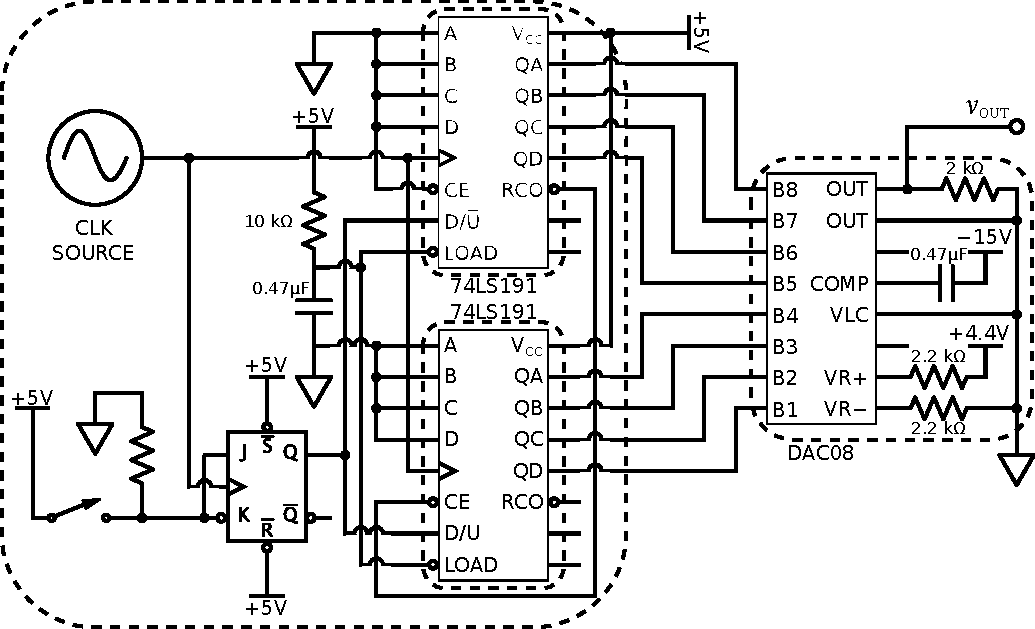
\includegraphics[width=.85\textwidth]{../E12/latex/DAC.pdf}
	\caption{}
	\label{cir12:DAC}
\end{figure}

Inseriamo dunque il DAC all'uscita del circuito discusso al paragrafo precedente come in Figura \ref{cir12:DAC} (dove per uscita intendiamo i valori di 0 e 1 logico in uscita dai due contatori). Essendo l'uscita di un contatore, il valore di tensione che ci aspettiamo di osservare sarà variabile (forma a dente di sega) dallo zero ad un valore impostabile. Per trovare tale valore bisogna tener conto del fatto che questo integrato lavora con correnti di riferimento. Per impostarla basta porre una corrente entrante al piedino 14: nel nostro caso abbiamo utilizzato una corrente
$$I_{rif}=\frac{4.4 \si{\volt}}{2.2\si{\kilo\ohm}} = 2 \si{\milli\ampere}$$
che ci permette di calcolare la corrente in uscita di fondo scala come (con n numero di bit, cioè 8)
$$I_{fs}=\frac{2^n - 1}{2^n} I_{ref} = \frac{7}{8} I_{ref}= 1.75 \si{\milli\ampere}$$
Dunque se poniamo all'uscita del DAC una resistenza di $2 \si{\kilo\ohm}$\footnote{Il costruttore richiedeva l'utilizzo di resistenze di valore più elevato; ma, vista l'impedenza in entrata dell'oscilloscopio, se avessimo inserito tale valore avremmo fatto passare corrente anche nell'oscilloscopio, rompendo l'approssimazione di partitore all'uscita.} messa a comune, ai suoi capi la caduta di tensione a fondo scala sarà di circa $3.5 \si{\volt}$. Come si vede nel grafico in Figura \ref{fig12:sega}, il valore atteso così calcolato è rispettato: infatti, il valore minimo di tensione ottenuto è stato di $-3.5 \si{\volt}$ (se colleghiamo l'oscilloscopio a $I_{out}$ la corrente è entrante nel DAC).

\begin{figure}[htpc]
\centering
	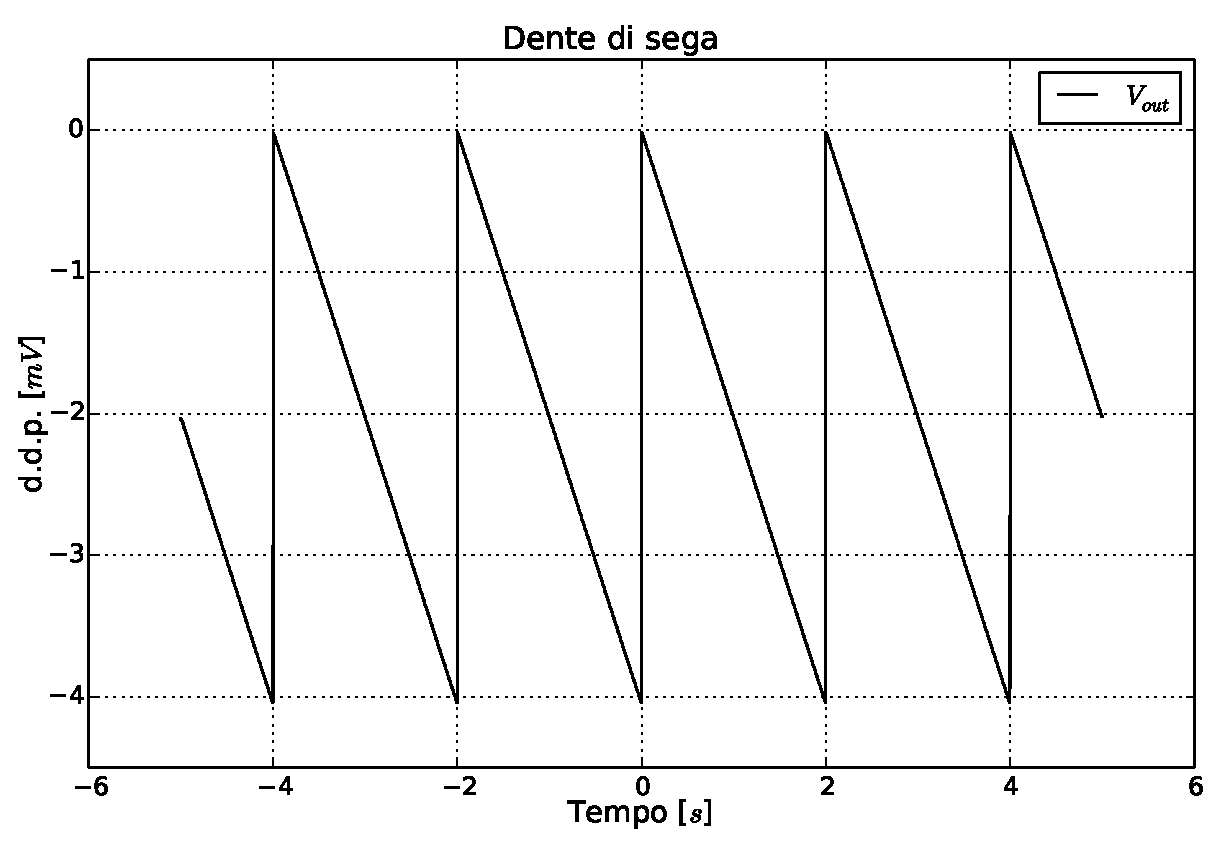
\includegraphics[width=.65\textwidth]{../E12/latex/sega.pdf}
	\caption{}
	\label{fig12:sega}
\end{figure}

Se vogliamo invece ottenere una forma d'onda triangolare dobbiamo far si che, al posto dell'interruttore per controllare la discesa e la salita, ci sia un dispositivo che inverta il valore logico in entrata nel JK quando c'è un massimo o un minimo. A tal fine, ci viene in aiuto un piedino dell'integrato che diventa uno nel massimo e nel minimo del segnale: ponendolo come clock di un JK in modalità toggle, questo invertirà Q sul fronte di salita (appunto quando c'è un massimo o un minimo).

\begin{figure}[htpc]
\centering
	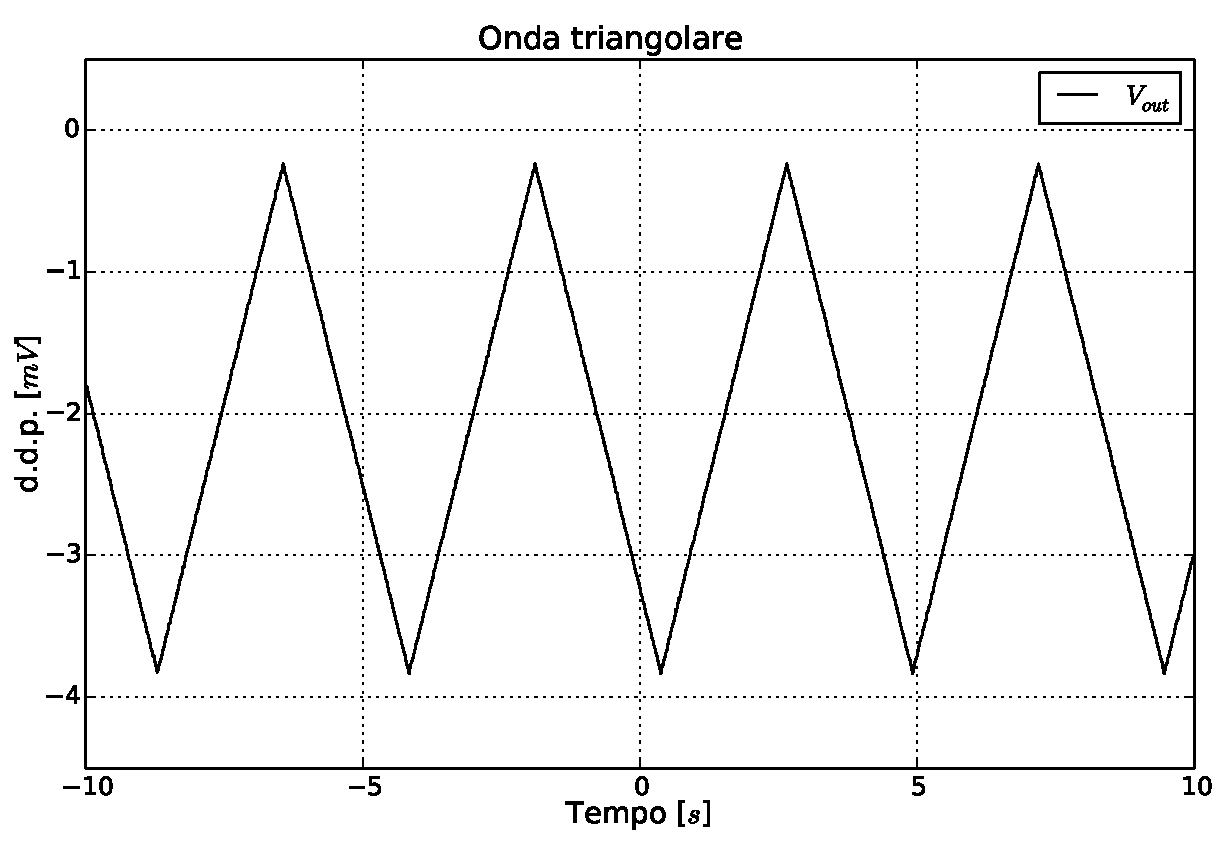
\includegraphics[width=.65\textwidth]{../E12/latex/triangolare.pdf}
	\caption{}
	\label{fig12:triangolare}
\end{figure}